\documentclass[12pt]{article}
\usepackage[utf8]{inputenc}
\usepackage{cmap}
\usepackage[T2A]{fontenc}



\usepackage{amssymb,amsfonts,amsthm,amsmath,mathtext,cite,enumerate,float}
\usepackage[russian, english]{babel}
\usepackage{graphicx}
\usepackage{tabularx}

\usepackage{enumerate}
\usepackage{fancyhdr}
\usepackage{a4wide}
\usepackage{cite}

\usepackage{caption}
\usepackage{subcaption}
\usepackage{multicol}
\usepackage{multirow}
\sloppy
\iffalse
Что защищается в работе:
    1. Предлагаемая архитектура должна базироваться на DARTS и быть не хуже в плане широты возможных моделей
    2. MLP --- поддерижвается
    3. Bayesian
    4. ??? Регуляция температуры
    5. ??? Параметр сложности модели
    Теорема Скляра
    
    1. Прописать цели
    2. Определения
    3. Связь
\fi
%\renewcommand{\headrulewidth}{0pt}
\DeclareMathOperator*{\argmin}{arg\,min}
\DeclareMathOperator*{\argmax}{arg\,max}
\begin{document}
\section{Цели работы}
Основная цель работы --- предложить метод выбора оптимальной структуры модели на основе байесовского вывода.
Предполагается, что предложенный метод будет работать не хуже существующих невероятностных методов (в плане accuracy наиболее вероятных параметров).
При этом такая модель будет более устойчива к возмущениям параметров/объектов, а также будет позволять прореживать блоки параметров на основании вероятностных оценок, полученных при поиске структуры.

Основныые требования к методу:
\begin{enumerate}
\item Метод должен быть сопоставим с методами, предложенными Zoph et al.
\item Метод должен позволять проводить поиск не только CNN, но и полносвязных сетей.
\item Метод должен быть эффективен по ресурсами.

\end{enumerate}
\newpage
\section{Обозначения}

\begin{table}[tbh!]
\small
\begin{tabularx}{\textwidth}{|X|p{1.5cm}|p{1.5cm}|X|p{1.5cm}|}
\hline
\multicolumn{5}{c}{Выборка и пр.}\\\hline
\bf Что & \bf Обозна- чение & \bf Простр. & \bf Что делает & \bf С чем связано  \\ \hline \hline

  Выборка & $\mathfrak{D}$ & - & - & $\mathbf{X}, \mathbf{y}$ \\ \hline
  Объекты & $\mathbf{X}$  &  $\mathbb{R}^{m \times n}$ & - & $\mathfrak{D}$   \\ \hline
  Метки & $\mathbf{y}$  &  $\mathbb{R}$ или $Z$ & - & $Z, \mathfrak{D}$   \\ \hline
  Количество классов & $Z$ & $\mathbb{Z}$ & - & $\mathbf{y}$ \\ \hline
\multicolumn{5}{c}{Модель (как граф)}\\\hline
  Нелинейная функция & $\mathbf{o}$ & - & Нелинейно отображает объекты внутри сети & - \\ \hline
  Множество нелинейных функций & $O$ & - & Набор возможных нелинейных функций для каждого элемента сети & $\mathbf{o}, \mathbf{f}$ \\ \hline
  Вершина графа & $v$ & $\mathbb{N}$ & Определяет операция над выборкой. Число определяет размерность объекта после прохождения операции & $V$ \\ \hline
  Множество вершин & $V$ & - & Множество возможных операций над выборкой. Каждая операция определяется своей матрицей, размерность которой соотвествует числу $v \in V$ & $v, d, \mathbf{f}$ \\ \hline
  Число вершин & $d$ - & - & $V$ \\ \hline
  Ребро графа & $e$ & $2^{d \times {d-1}}$ & Определяет наличие нелинейной функции, идущей от одной вершины к другой & $V$ \\ \hline
  %Валентность графа & $K$ & $\mathbb{N}$ & Максимальная степень вершины: сколько нелинейых операций может идти к одной вершине & $\mathbf{f}$ \\ \hline
  Модель & $\mathbf{f}$ & $E \to O$ & Отображение из ребра графа в нелинейную операцию & $E, O$ \\ \hline
  Множество моделей & $\mathfrak{F}$ & - & Множество моделей для заданного графа & $\mathbf{f}, V, E$ \\ \hline
  
\end{tabularx}
\end{table}


\begin{table}[tbh!]
\small
\begin{tabularx}{\textwidth}{|X|p{1.5cm}|p{1.5cm}|X|p{1.5cm}|}
\hline
\multicolumn{5}{c}{Модель (как вероятностная модель)}\\\hline
\bf Что & \bf Обозна- чение & \bf Простр. & \bf Что делает & \bf С чем связано  \\ \hline \hline
Параметры для одной вершины & $\mathbf{w}$ & $\mathbb{R}^{v}$ & & $v, \mathbf{W}$ \\ \hline 
Вектор параметров модели & $\mathbf{W}$ & - & Все параметры модели & $\mathbf{w}, \mathbf{f}$ \\ \hline
Структура для вершины, бинарный вектор с одной единицей & $\gamma$ & $2^{|O|}$ & Определяет веса нелинейных операций, входящих в веришну & $\boldsymbol{\Gamma}, v$ \\ \hline
Структура для модели & $\boldsymbol{\Gamma}$ & - & Определяет все веса нелинейных операций в модели & $\gamma$ \\ \hline
Ковариация параметров & $\mathbf{A}^{-1}$ & $\mathbb{R}^n$ & Определяет prior для параметров & $\mathbf{W}$ \\ \hline
Концентрация & $\alpha$  & $\mathbb{R}$ & Определяет prior для структуры & $\boldsymbol{\Gamma}$ \\ \hline
 
\multicolumn{5}{c}{Вариационный вывод}\\\hline
\bf Что & \bf Обозна- чение & \bf Простр. & \bf Что делает & \bf С чем связано  \\ \hline \hline
Вариационное распределение параметров модели & $q_\mathbf{w}$ &  - & Аппроксимирует апостериорное распределение & $\mathbf{A}^Q, \boldsymbol{\mu}$ \\ \hline
Среднее распределения параметров & $\boldsymbol{\mu}$ & - & - & $\mathbf{A}^Q, q_\mathbf{w}$ \\ \hline
Вариационное распределение параметров структуры & $q_\gamma$ & - & Аппроксимирует апостериорное распределение & $\mathbf{g}, \tau$ \\ \hline
Параметры распределения гумбель-софтмакс & $\mathbf{g}$ & - & - & $q_\gamma$ \\ \hline
Параметр температуры гумбель-софтмакс & $\tau$ & - & - & $q_\gamma$ \\ \hline

\multicolumn{5}{c}{Оптимизация}\\\hline
Функция потерь & $L$ &-& Оптимизируемая функция & $Q, \boldsymbol{\theta}, T$ \\ \hline 
Функция валидации & $Q$ & - & Оптимизируемая по гиперпараметрам функция & $L, \mathbf{h}, T$\\ \hline
Оптимизируемые параметры & $\boldsymbol{\theta}$ & - & - & $L, T$ \\ \hline
Оптимизируемые гиперпараметры & $\mathbf{h}$ & - & - &  $Q, T$ \\ \hline
Оператор оптимизации & $T$ & - & - &$L,Q$ \\ \hline
Количество итераций & $\eta$ & - & - & $T$ \\ \hline

\end{tabularx}

\end{table}
\clearpage
\begin{figure}[TBPH!]
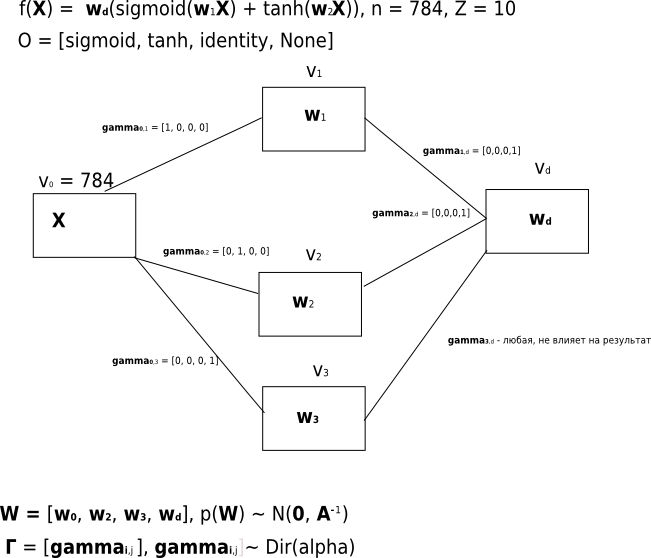
\includegraphics[width=\textwidth]{model_search.png}
\end{figure}
 

\clearpage
\section{Постановка задачи}
Задана выборка  \begin{equation}\label{eq:dataset}\mathfrak{D} = \{(\mathbf{x}_i,y_i)\}, i = 1,\dots,m,\end{equation} состоящая из множества пар <<объект-метка>> $$\mathbf{x}_i \in \mathbf{X} \subset \mathbb{R}^n, \quad {y}_i \in \mathbf{y} \subset \mathbb{Y}.$$ Метка ${y}$  объекта $\mathbf{x}$ принадлежит либо множеству: ${y} \in \mathbb{Y} = \{1, \dots, Z\}$ в случае задачи классификации, где $Z$ --- число классов, либо некоторому подмножеству вещественных чисел ${y} \in \mathbb{Y}  \subseteq \mathbb{R}$ в случае задачи регрессии. Определим множество архитектур моделей глубокого обучения для дальнейшего выбора оптимальной. 

\textbf{Определение} Функция $\mathbf{o}$ называется $n_1,n_2$ - допустимой, если для вектора $\mathbf{x} \in \mathbb{R}^{n_1}$ функция $\mathbf{o}$ определена и $\mathbf{o}(\mathbf{x}) \in \mathbb{R}^{n_2}$.


\textbf{Определение} Пусть задан вектор натуральных чисел  $V = [v_0, v1,\dots,v_d]$ и множество (возможно пустых) ребер $E$.
Пусть также задано множество нелинейных функций ${O}$, такое что нулевая функция лежит в этом множестве.
Соответствие $\mathbf{f}: E \to O$ будем называть моделью, если оно удовлетворяет условиям:
\begin{enumerate}
\item $\text{deg}^{+}({v}_0) = 0$
\item $\text{deg}^{-}({v}_d) = 0$.
\item Для каждого ребра $e$ между вершинами $v_i,v_j$ определена $v_i, v_j$-допустимая операция $\mathbf{o} \in O$.  
\end{enumerate}

\textbf{Определение} Параметрами модели (носителем?) $\mathbf{f}$, соответствующей графу $<V,E>$ с множеством операций $O$ будем называть вектор матриц $\mathbf{W} = [\mathbf{w}_1, \dots, \mathbf{w}_d]$ и бинарным множеством векторов, соответствующих ребрам графа $<V,E>$  $\boldsymbol{\Gamma} = \{\boldsymbol{\gamma}_{i,j}: (v_i,v_j) \in E \}, \boldsymbol{\gamma}_{i,j} \in \mathbb{R}^{|O|}$, т.ч. $\forall \gamma \in \boldsymbol{\Gamma}: ||\gamma||_1 \leq 1$.

Результатом функции $\mathbf{f}(\mathbf{x})$ будем полагать рекуррентное выполнение операций над $\mathbf{x}$ с выполнением обхода от вершины $v_0$:
\[
    f_0(\mathbf{x}) = \mathbf{x},
\]
\[
    f_i(\mathbf{x}) = \sum_{j: (j,i) \in E} \sum_{k = 1}^{|O|} {\gamma}^k_{i,j} \mathbf{o}_{k}  (\mathbf{w}_i f_j(\mathbf{x})). 
\]

Пусть для модели определено правдоподобие: $p(\mathbf{y}|\mathbf{W},\boldsymbol{\Gamma}, \mathbf{X})$. Пусть также задано априорное распределение параметров модели $\mathbf{W}$:
\[
    \mathbf{W} \sim \mathcal{N}(0, \mathbf{A}^{-1}), \quad \boldsymbol{\Gamma} \sim \text{Dir}(\alpha),
\]
где $\mathbf{A}^{-1}$ --- диагональная матрица гиперпараметров, $\alpha$ --- гиперпараметр концентрации весов параметров.

\textbf{Определение} Сложностью модели $\mathbf{f}$ назовем правдоподобие модели: 
\begin{equation}
\label{eq:evidence}
	p(\mathbf{y}|\mathbf{X},\mathbf{A},\alpha) = \int_{\mathbf{W}, \boldsymbol{\Gamma} } p(\mathbf{y}|\mathbf{X},\mathbf{W},  \boldsymbol{\Gamma})p(\mathbf{w}|\mathbf{A})p(\boldsymbol{\Gamma}|\alpha)d\mathbf{W}d\mathbf{\Gamma}.
\end{equation}


\textbf{Определение} Пусть заданы множество вершин $V$, множество операций $O$. Обозначим за $\mathfrak{F}(V,E,O)$ множество всех моделей для заданных $V,O$.
Модель $\mathbf{f}$ назовем оптимальной, если достигается максимум интеграла:
\[
    \mathbf{f} = \argmax_{\mathbf{f}' \in \mathfrak{F}(V,E,O)}\max_{\mathbf{A}} p(\mathbf{y}|\mathbf{X},\mathbf{A},\alpha).
\]

\newpage

\section{Вариационный вывод}
Введем два аппроксимирующих параметрических распределения: 
$$
q_\mathbf{w} \sim \mathcal{N}(\boldsymbol{\mu}, \mathbf{A}_q^{-1}) \approx p(\mathbf{W}|\mathbf{X}, \mathbf{y}, \mathbf{A}, \boldsymbol{\Gamma}),
$$
$$
q_\gamma \sim \text{Gumbel-Softmax}(\mathbf{g}) \approx p(\boldsymbol{\Gamma}|\mathbf{X}, \mathbf{y}, \mathbf{A}, \alpha).
$$

Пусть $L$ --- вариационная оценка правдоподобия:
\[
    L = \text{log} p(\mathbf{y}|\hat{\mathbf{W}}, \hat{(\boldsymbol{\Gamma}}) - \text{KLD}(q_\gamma||p(\boldsymbol{\Gamma})) - \text{KLD}(q_\mathbf{W}||p(\mathbf{W})).
\]

Пусть $Q$ --- потеря на валидации. Требования к функции:
\begin{enumerate}
\item Должна не противоречить максимизации ELBO.
\item Максимизация $Q$ должна вести к минимизации концентрации $\alpha$.
\item Слагаемое a_KL - поощряет сложность
\item Слагаемое D_KL(Q||P) для каждого шага - поощряет поиск новы структур
\end{enumerate}

Итого:
\begin{enumerate}
\item Хотим Add-Del: варьируем a_KL
\item Хотим честный sgd --- отключаем все
\item Хотим полный переор --- D_KL(Q||P)
\item Хотим ЛАссо --- фиксируем прайар
\item Хотим генетику --- видимо переходим к Ланжевену
\end{enumerate}

Пусть $\boldsymbol{\theta}$ --- параметры распределений $q_\mathbf{w}$ и $q_\gamma$:
\[
    \boldsymbol{\theta} = [\boldsymbol{\mu}, \mathbf{A}_q^{-1}, \mathbf{g}].
\] 

Пусть $\mathbf{h}$ --- параметры априорных распределений, а также гиперпараметры распределений  $q\mathbf{w}$ и $q_\mathbf{g}$:
\[
    \mathbf{h} = [\mathbf{A}, \alpha, \tau],
\]
где $\tau$ --- температура Гумбель-софтмакс распределения.



Сформулируем задачу поиска оптимальной модели как двухуровневую задачу.
\begin{equation}
\label{eq:optim}
	\hat{\mathbf{h}} = \argmax_{\mathbf{h} \in \mathbb{R}^h} Q( T^\eta(\boldsymbol{\theta}_0, \mathbf{h})),
\end{equation}
где $T$ --- оператор оптимизации, решающий задачу оптимизации:
\[
    L(T^\eta(\boldsymbol{\theta}_0, \mathbf{h})) \to \min.
\]

https://arxiv.org/pdf/1704.03003.pdf

\section{Нерешенные вопросы}
\begin{enumerate}
\item В работе Zoph et al. структуры оптимизируется с ограничением, что сеть является цепочкой повторяемых подмоделей. Таким образом, уменьшается количество возможных вариантов оптимизации и затраты по ресурами. В данной версии постановки задачи ограничений нет.
\item Кто отвечает за оптимизацию гиперпараметра $\alpha$. Кажется, что он должен быть фиксированным, но это противоречит байесовскому подходу.
\item Как регуляризовать путь оптимизации параметров.
\item Накладываем ли мы ограничения на степень вершин вычислительного графа?
\item Возможно потербуется как-то учитывать те параметры, которые не вошли в итоговый граф.
\end{enumerate}
\end{document}  
